\documentclass[11pt]{article}

\usepackage[english]{babel}
\usepackage[utf8]{inputenc}
\usepackage{amsmath}
\usepackage{amssymb}
\usepackage{graphicx}
\usepackage[colorinlistoftodos]{todonotes}
\usepackage{listings,multicol}
\usepackage{textcomp}
\usepackage{hyperref}
\usepackage{longtable}

\setlength{\oddsidemargin}{0.5cm} \setlength{\evensidemargin}{0cm}
\setlength{\textwidth}{16cm} \setlength{\textheight}{23cm}
\setlength{\topmargin}{-0.5cm}
\textheight 21.5cm

\usepackage{pgfplots}
\pgfplotsset{compat=1.6}

\pgfplotsset{soldot/.style={color=blue,only marks,mark=*}} \pgfplotsset{holdot/.style={color=blue,fill=white,only marks,mark=*}}


\usepackage[numbered,framed]{matlab-prettifier}
\lstMakeShortInline"
\lstset{
  style              = Matlab-editor,
  %basicstyle         = \mlttfamily,
  escapechar         = ",
  mlshowsectionrules = true,
}



\begin{document}

\title{L7 NUMERICO 220023-220138 UBB}

{\begin{minipage}{2cm}
\hspace*{1cm}
\includegraphics[width=0.6\textwidth]{escubo-ubb.eps}
\end{minipage}
\begin{minipage}{12cm}
\small
{\bf \rm 
{
\begin{center}
{\footnotesize UNIVERSIDAD DEL B\'IO-B\'IO} \\
{\scriptsize FACULTAD DE CIENCIAS}  \\
{\scriptsize DEPARTAMENTO DE MATEM\'ATICA}  \\
{\scriptsize Profesor:  Franco Milanese}\\
{\scriptsize Primer Semestre de 2016}
\end{center}
}}
\end{minipage}}
{\begin{minipage}{2cm}
\hspace*{-0.5cm}\vspace*{-0.05cm}
\includegraphics[width=0.7\textwidth]{escudo-dmat.eps}
\end{minipage}}

\hspace*{-1,5cm}\rotatebox[origin=c]{90}{\begin{picture}(0,0)
\put(0,7){\makebox(9,-13)[l]{\hspace*{-6.5in} \bf \it Departamento de Matem\'atica - Universidad del B\'io-B\'io - 2016}}
\end{picture}}


\vspace*{0.5cm} \centerline {\bf\underline{Laboratorio 7, M\'etodos Num\'ericos I 220023-220138}}
\centerline{\textrm{Semana 6 de junio de 2016.}}  \vspace{0.2cm}

% \textbf{Nombre:} \hspace{0.5\textwidth}\textbf{Carrera:}
% \vspace{0.1cm}
% \textbf{Profesor:}\hspace{0.5\textwidth} \textbf{ RUT:}
%  \begin{center}
%  \begin{tabular}{||p{2cm}|p{2cm}|p{2cm}||}
%  \hline
%  Pregunta 1 &  Pregunta 2 &     Total\\
%  \hline

%   \vspace{1.5cm} & &       \\
%  \hline
%  \end{tabular}
%  \end{center}
% Enviar documentos solicitados en el formato solicitado a \textbf{veranonumerico@gmail.com}.

\section{E.D.O. y P.V.I.}
Una E.D.O. de primer orden en la cual se exige que la funci\'on soluci\'on pase por un punto es un Problema de valores iniciales, estos se escriben de la forma
$$
\begin{array}{c|}
y'(x)=f(x,y(x))\\
y(x_0)=y_0\\
\hline
\end{array}
$$
por ejemplo
$$
\begin{array}{c|}
y'(x)=y(x)\\
y(0)=1\\
\hline
\end{array}\,,
\quad 
\begin{array}{c|}
y'(x)=sin(x)\\
y(1)=2\\
\hline
\end{array}\,,
\quad 
\begin{array}{c|}
y'(x)=cos(x)+y(x)\\
y(-1)=1\\
\hline
\end{array}\,,
$$
son  P.V.I. de orden uno que contienen una E.D.O. Estos problemas tienen por soluci\'n funciones de una variable $y(x)$ que satisfacen sus E.D.O. y la condici\'on inicial.

Una E.D.O. se dice de orden superior si esta incluye derivadas de orden mayor o igual que dos en su expresi\'on. Por ejemplo
$$
y''(x)+P(x)y(x)=F(x)
$$
es una E.D.O. de orden dos. Mediante sustituciones toda E.D.O. de orden superior se puede reescribir como un sistema de E.D.O. de orden uno. A modo de ejemplo la E.D.O.
$$
\begin{array}{c|}
2x''(t)-x'(t)-3x(t)=cos(t) \\
\hline
\end{array}
$$
se transforma en el sistema
$$
\begin{bmatrix}
u_1(t)\\
u_2(t)
\end{bmatrix}'
=
\begin{bmatrix}
u_2(t) \\
\frac{cos(t)+3u_1(t)+u_2(t)}{2}
\end{bmatrix}
$$
con la sustituci\'on
$u_1(t)=x(t)$ y $u_2(t)=x'(t)$.

\subsection{Soluci\'on num\'erica de P.V.I.}
Entendemos por soluci\'on num\'erica de un P.V.I. como una colecci\'on de puntos que, en cierto sentido, son similares a los puntos de muestreo de una funci\'on soluci\'on de un P.V.I.

\subsubsection{M\'etodo de Euler o RK11}
Los siguientes c\'odigos muestran la implementaci\'on de los m\'etodos num\'ericos de m\'as bajo orden vistos en la teor\'ia del curso. El primero es el m\'etodo de Euler y el segundo el de Euler impl\'icito, ambos caen dentro de la categor\'ia de un m\'etodo Runge Kutta de grado y orden 1.

En particular, para resolver el P.V.I.
$$
\begin{array}{rl|}
y'(x)	&=sen(x)\\
y(0)	&=1\\
x		&\in[0,10]\\ \hline
\end{array}
$$
implementamos

\vspace{5mm}
\begin{minipage}{0.5\textwidth}
\begin{lstlisting}
h=0.1;  %Tamano de paso
x=0:h:10;   %Vector de nodos
y(1)=1;     %Condicion incial
for i=2:length(x)   %Euler explicito
   y(i)=y(i-1)+h*sin(x(i-1));
end
plot(x,y);  %Grafica de la solucion
\end{lstlisting}
\end{minipage}
\hspace{5mm}
\begin{minipage}{0.5\textwidth}
\begin{lstlisting}
h=0.1;  %Tamano de paso
x=0:h:10;   %Vector de nodos
y(1)=1;     %Condicion incial
for i=2:length(x)   %Euler implicito
   y(i)=y(i-1)+h*sin(x(i));
end
plot(x,y);  %Grafica de la solucion
\end{lstlisting}
\end{minipage}
la gr\'afica de estas implementaciones es, donde se observa el error de los m\'etodos.
\begin{center}
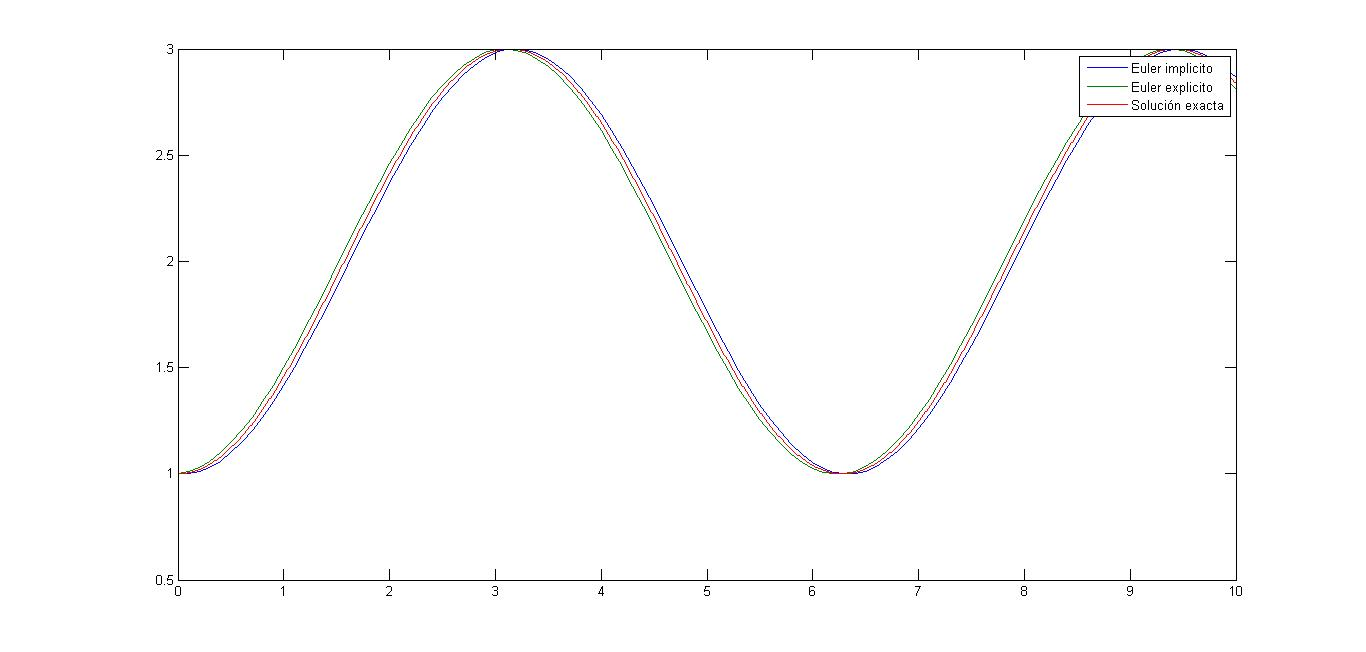
\includegraphics[width=0.85\textwidth]{./euler.jpg}
\end{center}

\section{M\'etodos num\'ericos para P.V.I. con funciones integradas en Matlab Matlab}

Matlab posee varias funciones para resolver P.V.I. y E.D.O. con m\'etodos num\'ericos. Algunas de estas son 
\begin{center}
\begin{tabular}{||p{0.15\textwidth}|p{0.15\textwidth}|p{0.15\textwidth}|p{0.45\textwidth}||}
\hline
{\bf Funci\'on 	}	&	{\bf Tipo de problemas} &	{\bf Precisi\'on} & {\bf Cuando usarla }\\ \hline
\texttt{ode45} 	&	No stiff	& Media			& Es posible usarla la mayoría de las veces. \texttt{ode45()} debe ser el primer intento de resolver una E.D.O.		\\
\texttt{ode23}  & No stiff		& Baja			& \texttt{ode23()} puede ser mas eficiente que \texttt{ode45()} en problemas que requieren poca precisi\'on.		\\
\texttt{ode113}	& No stiff 		& Baja a alta	& \texttt{ode113()} puede ser mas eficiente que \texttt{ode45()} en problemas que requieren mayor precisi\'on.		\\
\texttt{ode15s}	& Stiff			& Baja a media	& Debes intentar  \texttt{ode15s()} cuando \texttt{ode45()} falla o es ineficiente o se sospecha que el problema es stiff. \\
\texttt{ode23s}	&Stiff			& Baja			& \texttt{ode23s} puede ser mas eficiente que \texttt{ode15s()} en problemas que requieren baja precisi\'on. \\ \hline
\end{tabular}
\end{center}

La funci\'on \texttt{ode45()} opera bien con la mayor\'ia de los problemas de E.D.O. y en general estaba debe ser la primera elecci\'on de programas para resolver una E.D.O. Sin embargo, existen funciones como \texttt{ode23()} y \texttt{ode113()} que pueden ganar en eficiencia y precisi\'on a \texttt{ode45()}.

Algunas E.D.O. son del tipo stiff o son dif\'iciles de evaluar. Ser de tipo stiff es un t\'ermino que desaf\'ia una \'unica definici\'on precisa, pero esta sucede cuando hay alg\'una gran diferencia en las escalas de las variables involucradas en las E.D.O. Puedes identificar si un problema es stiff o no stiff, ocupando una funci\'on para problemas no stiff como \texttt{ode45()} y viendo si esta es incapaz de determinar la soluci\'on o si los c\'alculos son extremadamente lentos. 

\section{Ejemplos de uso de los solver num\'ericos de Matlab}
A continuaci\'on se ejemplifican marcos te\'oricos y el uso de las funciones de Matlab para implementar la soluci\'on de P.V.I. asociados a estos.

\subsection{Carga de un circuito RC}
Un circuito RC es diagramado seg\'un 
\begin{center}
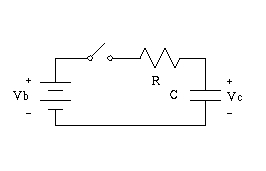
\includegraphics[width=0.5\textwidth]{cap1.jpg}
\end{center}
la carga del capacitor de este circuito depende de la diferencia de potencial el\'ectrico $V_{e}$ entregada por la fuente, la resistencia medida en Ohms $[\Omega]$ y la capacidad el\'ectrica del capacitor medida en Faradios $[\mu F]$. Este fen\'omeno es modelado por la ley de Kirchoff en el P.V.I
$$
\begin{array}{rl|}
C \frac{d}{dt}q(t)+\frac{q(t)}{R}	& =V_{e}(t) 	\\
					q(0)	&=q_0		\\ \hline
\end{array}
$$
las siguientes instrucciones de Matlab resuelven un problema de carga de un capacitor.
\begin{lstlisting}
%DATOS
V0=12;		%Voltaje de la fuente
R=1.5*10^(3);	%Resistencia electrica
C=4*10^(-3); 	%Capacidad del capacitor
tf=120;		%Tiempo final 
f=@(t,x) V0/C-x/(R*C); %Funcion del modelo

tiempo=[0 tf]; 	%intervalo de tiempo
q0=0;		%Carga inicial
[t,q]=ode45(f,tiempo,q0); %Solucion numerica
plot(t,q,'r')
xlabel('t')
ylabel('q');
title('Carga del condensador')
\end{lstlisting}
lo que genera la gr\'afica
\begin{center}
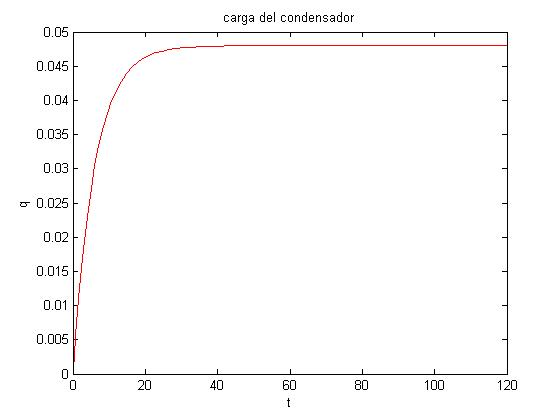
\includegraphics[width=0.5\textwidth]{eje1.jpg}
\end{center}

\subsection{Ecuaci\'on de conservaci\'on}
Del balance de masa en un sistema cerrado se deriva la relaci\'on
$$
\left(
\begin{minipage}{0.15\textwidth}
La razón de cambio de $Q(t)$,
\end{minipage}
\right)
=
\left(
\begin{minipage}{0.15\textwidth}
La razón a la que entra $Q(t)$
\end{minipage}
\right)
-
\left(
\begin{minipage}{0.15\textwidth}
La razón a la que sale $Q(t)$
\end{minipage}
\right).
$$
Este principio tiene varias aplicaciones en qu\'imica, f\'isica e ingenier\'ia.

\subsubsection{Disoluci\'on qu\'imica}

En qu\'imica una cantidad se suele medir en unidades de masa como son gramos, kilogramos o en cantidades como los moles. El volúmen se puede medir en litros, metros cúbicos u otras derivadas. La concentración de un soluto en un solvente se suele medir en unidades derivadas de estas como $[gr/L]$. El flujo de un solvente se puede medir en unidades de caudal como $[L/s]$ ó $[L/h]$.

Un tanque de $1500[L]$ contiene inicialmente $600[L]$ de agua con $1[Kg]$ de sal disuelto en ella. En un momento se le empieza a agregar agua a una raz\'on de $9[L/h]$ con una concentraci\'on de sal de $0.5[g/L]$. Si esta soluci\'on bien mezclada sale del tanque a $6[L/h]$, ¿Cuanta sal hay en el estanque cuando este se llena?.

Este problema se modela con el P.V.I.
$$
\begin{array}{rl|}
q'(t)	&= 0.5[g/L] \cdot 9[L/h] - \frac{q(t)}{600+3t} [g/h]\\
q(0)	&= 1000[g] \\ \hline
\end{array}
$$
donde $q(t)$ es la cantidad de sal en el estanque medida en gramos y $t$ es las horas transcurridad desde el inicio de la disoluci\'on.

El siguiente c\'odigo ejemplifica el uso de \texttt{ode45()} para la soluci\'on de este problema
\begin{lstlisting}
V0=600; %Volumen inicial
q0=1000;%Sal inicial
Qin=9;  %Caudal de entrada
Qout=6; %Caudal de salida
Cin=0.5;  %Concentracion de entrada
f=@(t,q) Qin*Cin-q/(V0+(Qin-Qout)*t)*Qout;
[t,q]=ode45(f,[0,120],q0);
plot(t,q,'-');
xlabel('tiempo medido en horas');
ylabel('cantidad de sal en el estanque');
title('Cantidad de sal en el estanque');
\end{lstlisting}
lo que genera la gr\'afica
\begin{center}
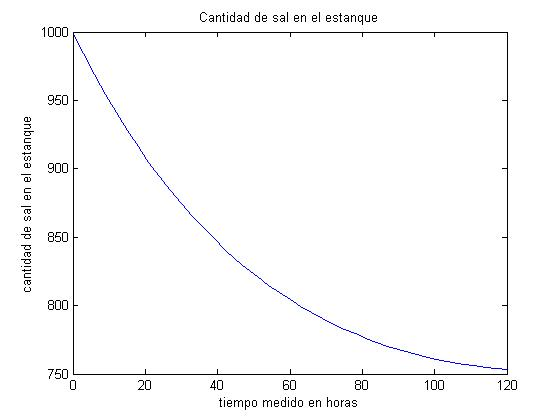
\includegraphics[width=0.5\textwidth]{eje2.jpg}
\end{center}

\subsection{Vaciado estanques}
El vaciado de un estanque es un proceso en regimen no estacionario debido a que tenemos una salida de masa de un sistema a una velocidad variable que dependerá de la altura del fluido en el estanque. Sin embargo, podemos suponer que mediante un balance de energía para una part\'icula de masa $m$ en el fluido
$$
\frac{1}{2}mv^2=mgh \rightarrow v=\sqrt{2gh},
$$
esta ecuaci\'on es conocida en hidrodin\'amica como la ley de Torricelli y establece la velocidad o flujo de salida $v$ de un estanque a trav\'es de un agujero que est\'a a una profundidad $h$. En la pr\'actica esta Ley no considera la prescencia de fuerzas disipativas, por lo que se corrije esta relaci\'on de la forma
$$
v=c\sqrt{2gh},
$$
donde $c$ se le llama coeficiente de descarga y $c\in[0,1]$.

Un estanque cilindrico de combustible de $5[m]$ de altura y $1000[L]$ de capacidad se encuentra lleno. Desde un momento se le hace una perforación circular de diametro $2[mm]$ en un cara inferior, por donde empieza a escurrir petr\'oleo. 

Este problema se modela con el P.V.I.
$$
\begin{array}{rl|}
\frac{1}{5}h'(t)	&= -\pi r^2\cdot \sqrt{2 g h(t)}\\
h(0)	&= 5[m] \\ \hline
\end{array}
$$
donde $h(t)$ es la altura de la columna de petr\'oleo en el estanque en funci\'on del tiempo $t$ medido en segundos. $r$ es el radio de la perforaci\'on y $g$ es la aceleraci\'on de gravedad.

El siguiente c\'odigo ejemplifica el uso de \texttt{ode45()} para la soluci\'on de este problema
\begin{lstlisting}
Ab=1/5; %Superficie de la base del estanque
Vtot=1; %Volumen total del estanque
r=0.002; %Radio de la perforacion
g=9.81;  %Aceleracion de gravedad
dh=@(t,h) -Ab/Vtot*pi*r^2*sqrt(2*g*h);
[t,h]=ode45(dh,[0,60*60*24*3],5);
plot(t,h)
xlabel('tiempo medido en s');
ylabel('altura en el estanque');
title('Vaciado de un estanque');
\end{lstlisting}
\begin{center}
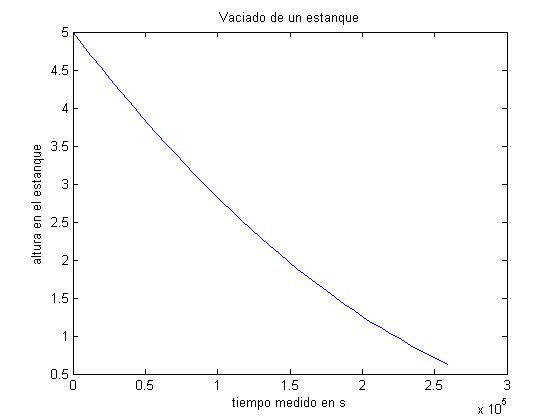
\includegraphics[width=0.5\textwidth]{eje3.jpg}
\end{center}

\subsection{Sistemas de ecuaciones diferenciales}
Distintos fen\'omenos pueden ser modelados usando sistemas de ecuaciones diferenciales. En general todos ellos modelan interacciones entre distintas magnitudes.

\subsubsection{Modelo de presa-depredador}
Suponga que $R(t)$ modela la cantidad de conejos en una isla y $F(t)$ modela la cantidad de zorros en una isla. Se puede suponer que existen ciertas relaciones entre los cambios en las poblaciones de conejos y zorros que podemos resumir en el sistema
$$
\begin{array}{cl}
R'(t)	&= a_1 R(t)- a_2 F(t)R(t) \\
F'(t)	&=-a_3 F(t)+ a_4 F(t)R(t),
\end{array}
$$
donde $a_1,a_2,a_3,a_4>0$ son constantes fijas que están relacionadas con la reproducci\'on de los zorros y conejos, y como uno alimentan a los otros.

En este contexto las condiciones iniciales $R(0)$ y $F(0)$ representan las poblaciones iniciales de conejos y zorros en la isla.

El siguien ejemplo muestra una modelaci\'on para ciertos par\'ametros y condiciones iniciales
\begin{lstlisting}
a1=0.4;
a2=0.37;
a3=0.3;
a4=0.05;
f=@(t,x)[a1*x(1)-a2*x(1)*x(2);-a3*x(2)+a4*x(1)*x(2)];
[t,f]=ode15s(f,[0,100],[3,1])
plot(t,f(:,1),t,f(:,2));
legend('Pob. conejos','Pob. zorros')
\end{lstlisting}
lo cual genera el gr\'afico
\begin{center}
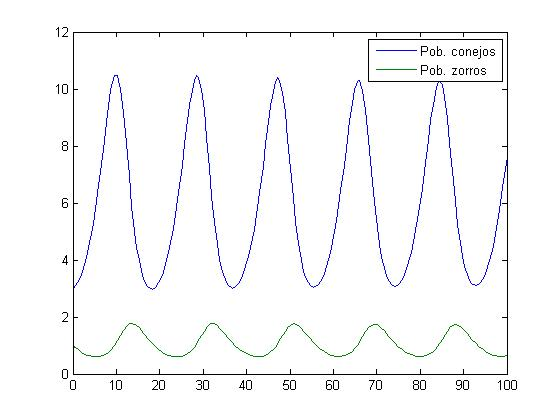
\includegraphics[width=0.5\textwidth]{eje4.jpg}
\end{center}

\subsubsection{Sistemas masa-resorte}
El P.V.I. 
$$
\begin{array}{rl|}
mx''+kx'+Rx	&=f(t)\\
x(0)	&=x_0\\
x'(0)	&=x_1\\\hline
\end{array}
$$
modela el movimiento de un sistema masa-resorte-amortiguador ideal cuya masa es $m[kg]$, su resorte es de constante $R[N/m]$ y el amortiguador es de coeficiente de difusión $k[N/(m/s)]$.

Este P.V.I. se puede replantear como el sistema de E.D.O.'s
$$
\begin{array}{rl}
u_1'(t)	&=u_2(t) \\
u_2'(t)	&=\frac{1}{m} \left( f(t)-ku_2(t)-Ru_1(t)\right)\\
u_1(0)	&=x_0\\
u_2(0)	&=x_1\\ \hline
\end{array}\,,
$$
el cual se genera mediante la sustituci\'on $u_1(t)=x(t)$, $u_2(t)=x'(t)$.  Matricialmente las E.D.O. del sistema se pueden pensar como
$$
\begin{bmatrix}
u_1(t)\\u_2(t)
\end{bmatrix}'
=
\begin{bmatrix}
u_2(t)\\\frac{1}{m} \left( f(t)-ku_2(t)-Ru_1(t)\right)
\end{bmatrix}
$$
esta es la forma de la funci\'on que se debe ingresar a Matlab para resolver el sistema.

El siguiente c\'odigo ejemplifica la modelaci\'on del movimiento de un resorte usando funciones de Matlab.
\begin{lstlisting}
k=1;
r=1;
m=1;
f=@(t,x) [x(2);1/m*(-k*x(2)-r*x(1))];
[t,f]=ode45(f,[0,20],[1,0]);
plot(t,f(:,1),'-k');
xlabel('tiempo');
ylabel('oscilacion');
title('Resorte amortiguado');
\end{lstlisting}
y genera la gr\'afica
\begin{center}
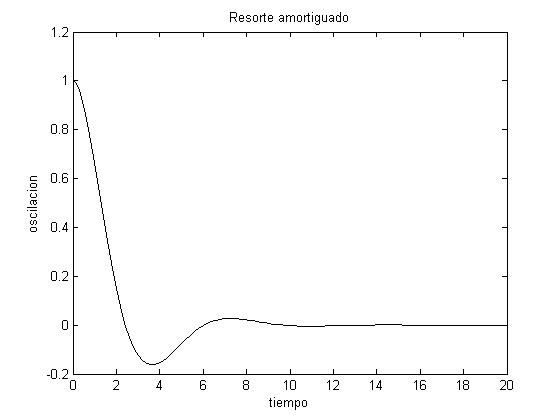
\includegraphics[width=0.5\textwidth]{eje5.jpg}
\end{center}

\newpage
\section{Ejercicios}
\begin{enumerate}
\item Programe el m\'etodo de Euler expl\'icito e Impl\'icito para resolver los problemas
\begin{multicols}{2}
\begin{enumerate}
\item
$\begin{array}{rl|}
y'	&=sen(2x)+y\\
y(0) &=0\\ \hline
\end{array}$
\item
$\begin{array}{rl|}
y'	&=cos(3x)\\
y(0)&=0\\ \hline
\end{array}$
\item
$\begin{array}{rl|}
y''-y'-2y	&=sen(2x)+y'\\
y(0)&=0\\
y'(0)&=0\\ \hline
\end{array}$
\end{enumerate}
\end{multicols}

\item La E.D.O
$$
y'=y^2-y^3
$$
modela el radio de una bola de fuego $y(t)$ en funci\'on del tiempo de combusti\'on. La idea es que este radio es proporcional a la superficie de la bola de fuego e inversamente proporcional a su volumen. Las llamas crecen r\'apidamente y, a medida que alcanzan su volumen final, dejan de crecer. 

Resuelva num\'ericamente el P.V.I.
$$
\begin{array}{rl|}
y' 		&=y^2-y^3 \\
y'(0) 	& \delta \\ \hline
\end{array}
$$
considerando $\delta=0.1$, $\delta=0.05$,$\delta=0.001$ y $\delta=10 ^{-8}$.

\item Un paracaidista de $80[kg]$ se suelta desde un avi\'on a una altura de $600[m]$. Despu\'es de $5[s]$ el paracaida se abre.

La altura del paracaidista, en funci\'on del tiempo, $y(t)[m]$ se modela por el P.V.I.
$$
\begin{array}{rl|}
y'' 	& = -g+\frac{1}{m}\alpha(t) \\
y(0)	& = 600\\
y'(0)	& 0\\ \hline
\end{array}
$$
donde $g=9.81[m/s^2]$ es la aceleraci\'on de gravedad, $m=80[kg]$ es la masa del paracaidista y $\alpha(t)$ es la resistencia del aire, la cual es proporcional al cuadrado de la velocidad del paracaidista, pero esta cambia cuando el paracaida se abre seg\'un
$$
\alpha(t)=
\begin{cases}
K_1\, y'(t)^2 , \quad \text{si} \quad t<5[s]\\
K_2\, y'(t)^2 , \quad \text{si} \quad t\geq 5[s]
\end{cases}.
$$
\begin{enumerate}
\item Calcule la soluci\'on anal\'itica en caida libre del paracaidista $(K_1=K_2=0)$. ¿Cuanto tiempo se demora el paracaidista en llegar a tierra?, ¿Cual es la velocidad del impacto?. Grafique la altura versus el tiempo.
\item Resuelva num\'ericamente considerando 
$$
K_1=1/15, \quad K_2=4/15.
$$
¿A qu\'e altura se abre el paracaida?, ¿Cuanto se demora en llegar al suelo?, ¿Cuál es la velocidad del impacto?. Grafique la altura versus el tiempo.
\end{enumerate}

\newpage
\item \textbf{Deflexiones de una viga}

Muchas estructuras se construyen mediante vigas o travesa\~{n}os y estas se distorsionan bajo su propio peso o por influencia de algunas fuerzas externas. 
     \begin{figure}[htp]
      \begin{center}
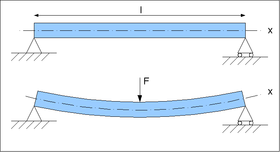
\includegraphics[width=0.5\textwidth]{./viga.png}
      \caption{\sl Deflexi\'on en una viga.}
      \end{center}
      \end{figure}
      
Supongamos que una viga de longitud $L$ es homog\'enea en su composici\'on y que tiene cortes transversales uniformes a su largo. En ausencia de cualquier carga en la viga, incluyendo su propio peso, la viga describir\'a una recta llamada eje de simetr\'ia. Si una carga se aplica a la viga, en forma perpendicular al eje de simetr\'ia, esta experimenta una deformaci\'on. La curva que describe la deformaci\'on de cada punto respecto al eje de simetr\'ia es llamada \textbf{curva de deflexiones} o \textbf{curva el\'astica}. En cierto sentido, la curva de deflexiones aproxima la forma de la viga.
     \begin{figure}[htp]
      \begin{center}
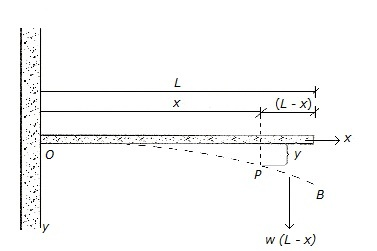
\includegraphics[width=0.5\textwidth]{./viga1.jpg}
      \caption{\sl Sistema coordenado en una viga y curva de deflexi\'on.}
      \end{center}
      \end{figure}

Suponga que el eje $x$ coincide con el eje de simetr\'ia de una viga y que la deflexi\'on es medida como funci\'on de la posici\'on del eje $x$, digamos $y(x)$. En la teor\'ia de elasticidad se tiene que
$$
EI y^{(iv)}(x)=w(x),
$$
donde $E$ es el m\'odulo de Young, $I$ es el momento de inercia de un corte transversal de la viga, ambas constantes que dependen de la geometr\'ia y material de la viga, mientras que $w(x)$ es la carga que hay en el punto $x$ de la viga.

La condiciones de contorno para la curvatura el\'astica cumplen un rol importante, y podemos clasificarlas en tres tipos de vigas

\begin{center}
\begin{tabular}{||c|c||}
\textbf{Extremos en la viga} & \textbf{Condiciones de frontera}  \\
\hline
Empotrados 	& $y=0$, $y'=0$ 	\\                                    
Libres		& $y''=0$, $y'''=0$	\\
Apoyados	& $y=0$, $y''=0$	 
\end{tabular}
\end{center}

\begin{enumerate}
\item
Encuentre la soluci\'on num\'erica que describa la deflexi\'on de una viga de largo $L$ empotrada en ambos extremos sujeta a una carga constante $w_0$.

Grafique la deflexi\'on de vigas de largo $1$ , $10$ y $100$ cuando $w_0=24\times 10^{-4}$.

\item 
Encuentre la soluci\'on num\'erica que describa la deflexi\'on de una viga de largo $L$ empotrada en un extremo y libre en el otro, sujeta a una carga constante $w_0$.

Grafique la deflexi\'on de vigas de largo $1$ , $10$ y $100$ cuando $w_0=24\times 10^{-5}$.

\item 
Encuentre la soluci\'on num\'erica que describa la deflexi\'on de una viga de largo $L$ empotrada en ambos extremos, sujeta a una carga $w(x)=w_0 x$.

Grafique la deflexi\'on de vigas de largo $1$ , $10$ y $100$ cuando $w_0=24\times 10^{-1}$.
\end{enumerate}


\end{enumerate}
\begin{thebibliography}{9}
\bibitem{Mo2} Moler, Cleve, Numerical Computing with MATLAB, S.I.A.M. Disponible en http://www.mathworks.com/moler/odes.pdf

\bibitem{S1} Shampine, L. F. and M. W. Reichelt, "The MATLAB ODE Suite," SIAM Journal on Scientific Computing, Vol. 18, 1997, pp. 1–22.

\bibitem{S2} Shampine, L. F., Gladwell, I. and S. Thompson, Solving ODEs with MATLAB, Cambridge University Press, Cambridge UK, 2003.

%\bibitem{MH} Heath, Michael, Scientific Computing: an introductory survey. McGraw Hill 2005.

%\bibitem{DB} de Boor, Charles, A Practical Guide to Splines, Springer-Verlag, New York, 1978.

% http://www.uam.es/personal_pdi/ciencias/barcelo/cnumerico/recursos/interpolacion.html

%\bibitem{H1} N. J. Higham, Accuracy and Stability of Numerical Algorithms, SIAM, Philadelphia, 2002
\end{thebibliography}

\end{document}
